\documentclass[]{spie}  %>>> use for US letter paper
%\documentclass[a4paper]{spie}  %>>> use this instead for A4 paper
%\documentclass[nocompress]{spie}  %>>> to avoid compression of citations

\renewcommand{\baselinestretch}{1.0} % Change to 1.65 for double spacing
\newcommand{\aap}{Astronomy \& Astrophysics}
\newcommand{\procspie}{Proc.\ SPIE}
\newcommand{\aspconf}{ASP Conf.\ Ser.}
\newcommand{\qjras}{QJRAS}
\newcommand{\ssr}{Space Science Reviews}

\newcommand{\ascl}[1]{\href{http://www.ascl.net/#1}{ascl:#1}}
\newcommand{\arxiv}[1]{\href{http://arxiv.org/abs/#1}{arXiv:#1}}
\newcommand{\doi}[1]{\href{http://dx.doi.org/#1}{doi:#1}}

\usepackage{amsmath,amsfonts,amssymb}
\usepackage{graphicx}
\usepackage[colorlinks=true, allcolors=blue]{hyperref}

\title{Investigating interoperability of the LSST Data Management software stack with Astropy}
% Jenness, Bosch, Owen, Parejko, Sick, Swinbank, de Val-Boro et al
\author[a]{Tim Jenness}
\author[b]{James Bosch}
\author[c]{Russell Owen}
\author[c]{John Parejko}
\author[a]{Jonathan Sick}
\author[b]{John Swinbank}
\author[b]{Miguel de Val-Borro}
\author[d]{Gregory~Dubois-Felsmann}
\author[e]{K-T~Lim}
\author[b]{Robert~H.~Lupton}
\author[b]{Pim~Schellart}

\affil[a]{LSST Project Management Office, Tucson, AZ, U.S.A.}
\affil[b]{Princeton University, Princeton, NJ, U.S.A.}
\affil[c]{University of Washington, Seattle, WA, U.S.A}
\affil[d]{Infrared Processing and Analysis Center, California Institute of Technology, Pasadena, CA, U.S.A.}
\affil[e]{SLAC National Laboratory, Menlo Park, CA, U.S.A.}

\authorinfo{Further author information: (Send correspondence to T.J.)\\T.J.: E-mail: tjenness@lsst.org}

% Option to view page numbers
\pagestyle{empty} % change to \pagestyle{plain} for page numbers
\setcounter{page}{301} % Set start page numbering at e.g. 301

\begin{document}
\maketitle

\begin{abstract}
  The Large Synoptic Survey Telescope (LSST) will be an 8.4\,m optical survey telescope sited in Chile and capable of imaging the entire sky twice a week.
  The data rate of approximately 15\,TB per night and the requirements to both issue alerts on transient sources within 60 seconds of observing and create annual data releases means that automated data management systems and data processing pipelines are a key deliverable of the LSST construction project.
  The LSST data management software has been in development since 2004 and is based on a C++ core with a Python control layer.
  The software consists of nearly a quarter of a million lines of code covering the system from fundamental WCS and table libraries to pipeline environments and distributed process execution.

  The Astropy project began in 2011 as an attempt to bring together disparate open source Python projects and build a core standard infrastructure that can be used by and built upon by the astronomy community.
  This project has been phenomenally successful in the years since it has begun and has grown to be the de facto standard for Python software in astronomy.
  Astropy brings with it considerable expectations from the community on how astronomy Python software should be developed and it is clear that by the time LSST is fully operational in the 2020s many of the prospective users of the LSST software stack will expect it to be fully interoperable with Astropy.

  In this paper we describe the overlap between the LSST science pipeline software and Astropy software and investigate areas where the LSST software provides new functionality.
  We also discuss the possibilities of re-engineering the LSST science pipeline software to build upon Astropy, including the option of contributing affiliated packages.
\end{abstract}

% Include a list of keywords after the abstract
\keywords{Astronomy Software, Python, Code Reuse}

\section{INTRODUCTION}
\label{sec:intro}  % \label{} allows reference to this section

One major component of the Data Management system\cite{2016_adassxxv_O3-1} for the Large Synoptic Survey Telescope (LSST)\cite{2008arXiv0805.2366I,2016SPIE-Kahn,2014SPIE.9145E..1AG} is a software pipeline capable of reducing LSST images to catalogs during both low-latency nightly and high-throughput data release processing.
This pipeline must be able to process data promptly from the 3.2~gigapixel camera\footnote{This equates to approximately 15\,TB per night. See \url{http://lsst.org/scientists/keynumbers} for additional numbers.} and issue alerts on transient sources within 60 seconds of observing.
It must also be able to efficiently process the 11 data releases that will be made during the ten year survey.

In addition to efficiency, the LSST pipelines must also provide unprecedented levels of control over systematic errors across a broad range of scientific domains.
Most consumers of LSST data will likely do no image processing of their own, and even those that do will rely heavily on catalogs generated by the LSST pipeline.
Furthermore, much of LSST data analysis is expected to happen in LSST's ``Level 3 Environment'', a combination of hardware and software that will allow scientists to run their own code and customized versions of LSST pipeline algorithms on LSST's middleware and hardware.
While algorithmically advanced pipelines and public catalog releases have become the norm for large surveys over the past 20 years, LSST's will thus be the first for which the software must be accessible to and usable by scientists outside the pipeline team.

The difficulty of sharing code between telescopes has long been a topic of discussion in the astronomy software community\cite{1998ASPC..145..142M,1999ASPC..172...11E,2001ASSL..266..163S,2002SPIE.4844..321E}.
Historically there have been some successes in fundamental libraries, such as SOFA\cite{2011SchpJ...611404H}, CFITSIO\cite{1999ASPC..172..487P} and wcslib\cite{2011ascl.soft08003C}, and in environments, such as IRAF\cite{1986SPIE..627..733T}, AIPS\cite{1996ASPC..101...37V} and Starlink\cite{1982QJRAS..23..485D}.
Despite these, there is still a tendency for a new project to embark on the creation of a new environment or software infrastructure if there are slight requirements mismatches and no external political will to adopt a specific software suite.
The growth in the Open Source software movement\cite{2006OpenSources} and recent explosion in support tools such as git and GitHub for code sharing\cite{2014IACWSLima}, makes the process of software reuse far easier than it has ever been.

The LSST data processing pipeline software has been in development as an open source project since 2004\cite{2004AAS...20510811A,2010SPIE.7740E..15A,2016_adassxxv_P056} and during these 12 years of development much has changed in the Python, C++ and astronomy software world.


\section{The LSST Science Pipeline Software}

As with other software developed in the early 2000s, such as CASA\cite{2012ASPC..461..849P}, the LSST science pipeline software is based on a C++ core with a Python control layer, where the Python/C++ interface layer is handled via SWIG\cite{beazley2003automated} bindings.
The general layout of the code is shown in Fig.~\ref{fig:layers}.
At the time of writing the LSST science pipelines codebase is split between C++ and Python with of order 105,000 lines of Python and 125,000 lines of C++\footnote{This total does not include comment or blank lines, nor does it include the 80,000 lines of Python and 1.6\,million lines of C++ generated for the SWIG wrappers.}.

\begin{figure} [t]
\begin{center}
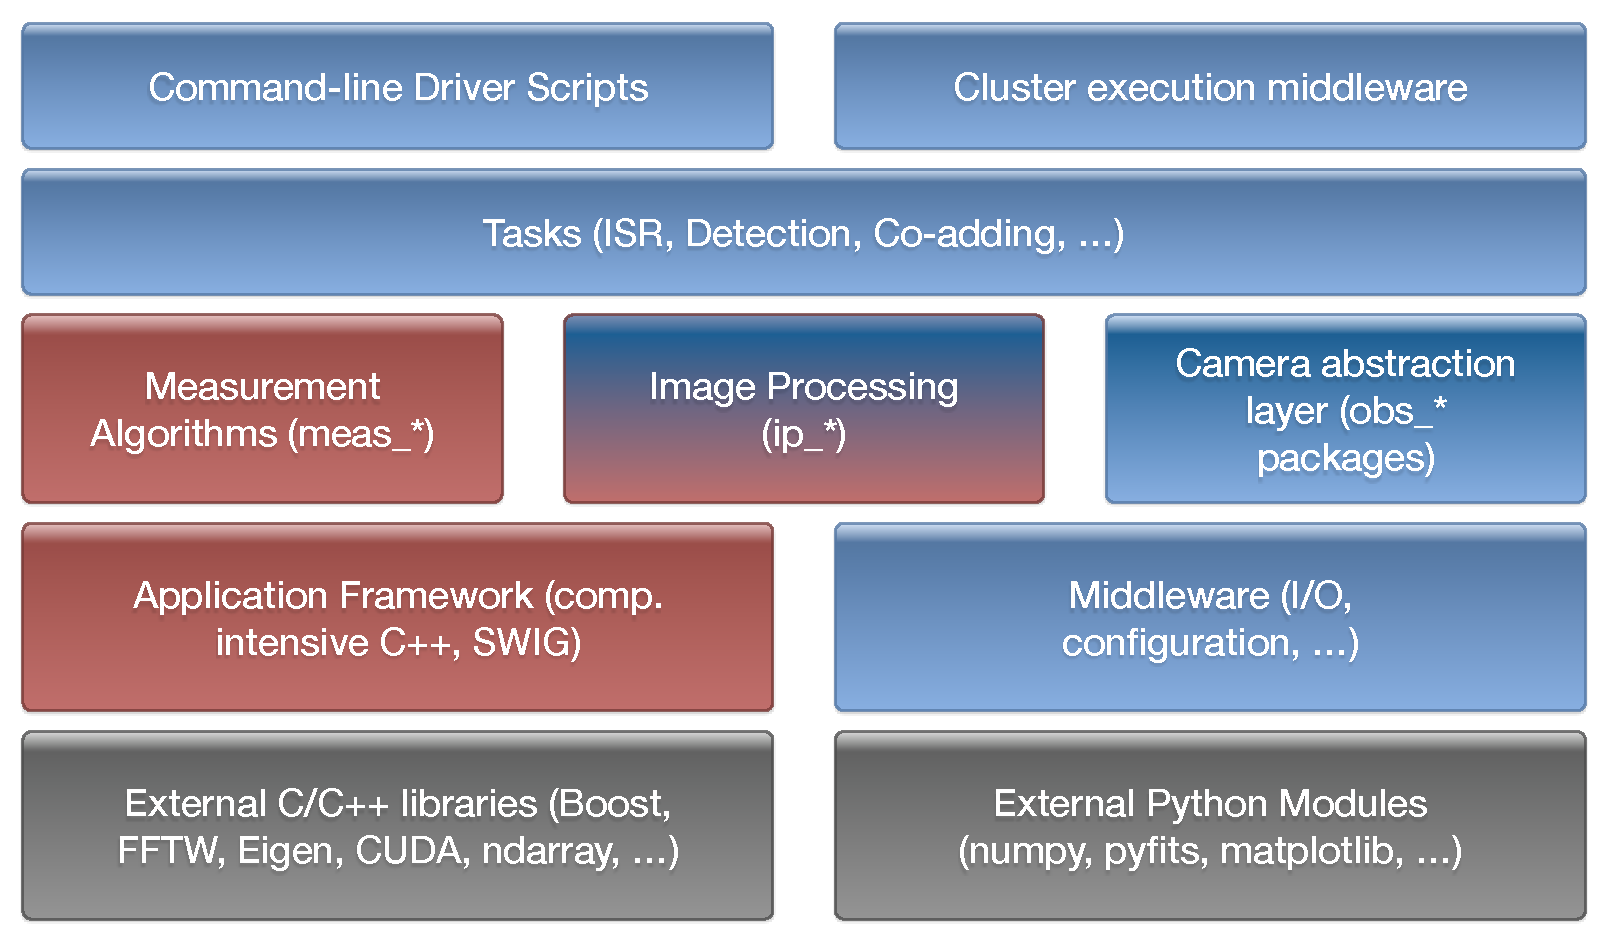
\includegraphics[height=5cm]{Software-Layers}
\end{center}
\caption[layers]
%>>>> use \label inside caption to get Fig. number with \ref{}
{\label{fig:layers}
Structure of the LSST data management software.
At the bottom there are external packages (black), on the lower left (red) are the computationally intensive packages that are mainly written in C++ with SWIG wrappers making the code available in Python, and the remainder (blue) are mostly Python.}
\end{figure}

The software is spread among many different root packages within the \texttt{lsst} namespace:

\begin{description}
\item[\textbf{afw}] These provide core LSST utility classes including geometric shapes, images, source detection, convolution and high-level exposure objects.

\item[\textbf{daf}] The data access framework, also known as \emph{the Data Butler}, provides an abstraction layer hiding data formats and locations from the user and providing them with standardized Python objects representing the data.

\item[\textbf{ip}] Low-level image processing algorithms such as instrument signature removal and image differencing.

\item[\textbf{meas}] Algorithms focused on processing individual sources in an image, including PSF modeling, WCS fitting, and source detection, deblending, and measurement.

\item[\textbf{obs}] Observatory plugins to teach the system how to handle files from different instruments.

\item[\textbf{pipe\_base}] Pipeline processing infrastructure. This allows discrete units of computation to be linked together to form pipelines.

\item[\textbf{pipe\_tasks}] High-level algorithms, including initial exposure-level processing and calibration, image coaddition (with sophisticated artifact rejection and coaddition of PSF models), and consistent multi-passband processing of coadds to measure colors.

\end{description}

The LSST code base currently contains additional components that are not of short-term interest for Astropy integration but might become so in the longer run.
These include the Data Butler and the Task framework.
The Butler is a client library for generic data access that abstracts away details of serialization, data storage, and data transport as well as providing facilities for handling simple versioning and time-based data access with validity ranges.
The Task framework provides a way of packaging science algorithms so that they can be executed in a data-parallel fashion, with further extensions to allow MPI-based tightly-synchronized execution.
The framework includes a Python-based configuration language that has default values, overrides from code as well as the end user, and hooks for validation of configured values.
In terms of overlap with Astropy and affiliate packages the \texttt{afw} and \texttt{meas} packages are most relevant for immediate investigation.

The algorithms in the LSST codebase are not yet at the level of scientific quality ultimately needed for LSST, but they are already being used to process data from the Hyper Suprime-Cam Survey on the Subaru telescope\cite{2012SPIE.8446E..0ZM}, one of the major precursors surveys for LSST, and generally represent the current state-of-the-art.


\section{Astropy}

Python has become the dominant programming language for astronomy\cite{2000ASPC..216...59G,2006ASPC..351..343H,2006ASPC..351..497K,2011ASPC..442..425G,2012SPIE.8451E..02J} and is now the default choice for new projects and for teaching.
The Astropy\cite{2013A&A...558A..33A} project grew out of a support mailing list in 2011 to become a very successful hub for the development of Python packages for astronomy.
At the time of writing Astropy consists of approximately 105,000 lines of Python code.
Astropy has two key approaches to drive adoption.
The first is to place generic astronomy code into the \emph{core} package that is brought in via \texttt{import astropy} to provide a solid, well-tested base for astronomy software development; the second is to support and encourage the concept of \emph{affiliated} packages, which use the \texttt{astropy} package and follow the same philosophy on distribution and openness.
Together these aim to provide a consistent environment of highly-usable, well-documented, easy-to-install code for astronomers trying to use Python in their research.

\section{Synergies}

The LSST project is constrained by the requirements of the funding agencies to deliver a data management system on schedule and on budget.
Involvement with Astropy is justifiable if it helps the project improve schedule or performance or if it improves community usability while not impacting deliverables.
It is also possible that making it easier for the community to adopt LSST algorithms can improve robustness of the code and find bugs earlier.
The community will be encouraged to try out the LSST software sooner if it integrates well with Astropy.
This is likely to significantly enhance utilization of the compute resources provided at LSST data access centers, what LSST calls the Level 3 processing system, during LSST operations resulting in a system that is more scientifically productive.

The Astropy and LSST software projects are both attempting to write astronomical software in Python that will benefit the community.
In this section we look at the areas code can be contributed by LSST to Astropy and where collaboration between LSST and Astropy can enhance both projects.
In Section~\ref{sec:lsstmods} we address the areas where LSST can benefit directly from improving interoperability with Astropy software.

\subsection{Generalized Word Coordinate Systems}

The James Webb Space Telescope (JWST)\cite{2006SSRv..123..485G} and LSST have requirements for accurate world coordinate conversions that cannot be represented in the current FITS World Coordinate Systems (FITS-WCS) framework\cite{2013ASPC..475...49H,2002A&A...395.1077C,2015A&C....12..133T} and none of the current extensions handling focal plane distortions\cite{2012SPIE.8451E..1MS,2012tpv} are suitably flexible.
This lack of flexibility in FITS-WCS has been a long standing issue and the Starlink AST library\cite{Berry201633} provides one solution to this problem that has been in use for nearly 20 years.
For JWST a pure-Python equivalent, the Generalized World Coordinate Systems (GWCS) package, is in development\cite{2016_P028_adassxxv} and is not yet part of Astropy but builds on the \texttt{astropy.modeling} framework.
LSST expects to require world coordinate transformations to be performed in the C++ layer for performance reasons, and this may preclude direct adoption of GWCS by LSST, given the performance limitations of a pure-Python implementation.
It would be beneficial to both parties if the future LSST WCS implementation and GWCS could interoperate easily.
We are therefore investigating a text-based serialization of WCS that could be usable as an interchange format.
AST currently supports a number of serialization schemes including multiple dialects of FITS headers, the International Virtual Observatory Alliance (IVOA)\footnote{\url{http://www.ivoa.net}} Space-Time Coordinate Linear String format (STC-S)\cite{2007ivoa.spec.1030R} for region handling\cite{2010ASPC..434..213B} and an internal text-based format.
GWCS can serialize to FITS-WCS and also into YAML\cite{2009yaml} using the Advanced Scientific Data Format (ASDF)\cite{2015A&C....12..240G}.
We have decided to investigate a common format that is based on YAML and the proposed new variant of STC, version 2.0.
STC-2\cite{2015ivoaSTC2} is an evolution of STC that includes support for chainable mappings and seems like it could be a suitable starting point for this investigation.
Both the Astropy and IVOA communities would benefit if such a standard could be established and it could be a significant factor in bringing together the competing distortion models currently in use in the FITS community.

\subsection{Region handling}

The handling of regions such as circles and polygons is not yet supported in Astropy core.
The Astropy affiliate \texttt{pyregions} package does have code for handling region files from the DS9 application\cite{2005ASPC..347..110J}, with some discussions concerning adopting the IVOA STC standard\cite{2007ivoa.spec.1030R} as a region serialization format.
In addition, the \texttt{photutils} affiliated package has some basic support for rasterizing analytic regions in pixel coordinates for photometry.
A new affiliate package \texttt{astropy.regions}\footnote{\url{https://github.com/astropy/regions}} hopes to unify this functionality and provide a consistent interface for all region operations in Astropy, with the expectation that this functionality will move to Astropy core once the interface stabilizes.

LSST's codebase actually includes two distinct geometry libraries:
\texttt{afw.geom} includes points, boxes, polygons and ellipses for Cartesian coordinate systems, while \texttt{sphgeom} provides similar geometric primitives in spherical polar coordinates.
These do not currently interoperate smoothly, reflecting the fact that they have thus far been used only in completely different components of the codebase.
Integrating these libraries will clearly be important for LSST in the future, suggesting that now is a perfect time for LSST and Astropy to collaborate on a new unified regions library.
LSST could provide mature implementations of individual geometry classes to such a collaboration, while Astropy brings serialization and visualization code as well as a broader sense of the requirements for a unified library.
A major challenge for a jointly-developed library is reconciling LSST's need for C++ geometry classes (with Python bindings) with Astropy's preference for pure Python for easier installation and maintenance.

\begin{figure}[t]
\begin{center}
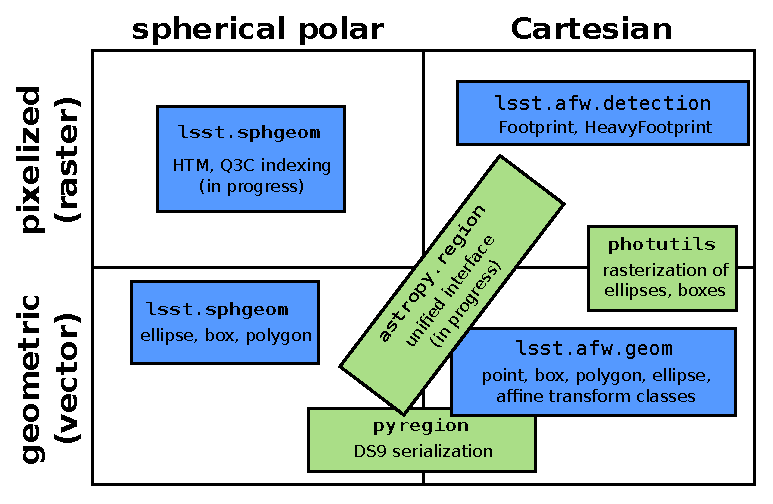
\includegraphics[width=0.5\textwidth]{regions}
\end{center}
\caption{Four ways of representing regions, and the approximate domains of the LSST (blue) and Astropy (green) packages for manipulating them.}
\label{fig:regions}
\end{figure}

STC-S is already being used to define sky regions in the VO community and is also understood by the GAIA visualization tool\cite{2009ASPC..411..575D} and Starlink software\cite{2010ASPC..434..213B,2014ASPC..485..391C}.
If Astropy and LSST cannot share sky-to-pixel region handling code directly, there is a possibility that STC could be adopted to allow interoperability.

\begin{figure} [t]
\begin{center}
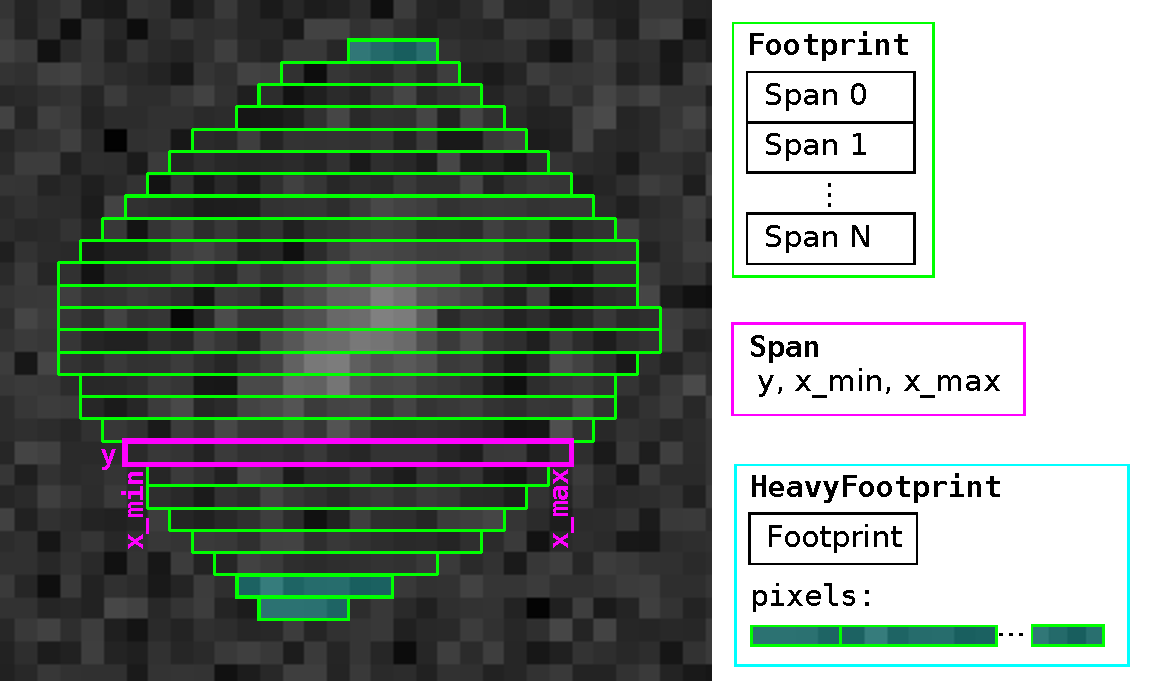
\includegraphics[width=0.5\textwidth]{footprint}
\end{center}
\caption[footprint]
%>>>> use \label inside caption to get Fig. number with \ref{}
{\label{fig:footprint}
LSST's \texttt{Footprint} data structure.
A \texttt{Footprint} describes a pixelized region as a sequence of \texttt{Spans}, each of which holds the y position and minimum and maximum x positions.
A \texttt{HeavyFootprint} combines a \texttt{Footprint} with the values of the pixels it covers by simply storing the pixels of each span back-to-back.}
\end{figure}

Most of the above work focuses on the lower half of Figure~\ref{fig:regions}, but Astropy's unified region plans also include rasterization to images (upper right corner).
Pixelizing LSST geometries instead typically involves yet another class: \texttt{afw.detection.Footprint} (Figure~\ref{fig:footprint}).
\texttt{Footprint} is a compact serialized representation of a mask, listing the pixel indices that contribute to the shape in rasterized order, using a run-length encoding algorithm to conserve space.
A \texttt{HeavyFootprint} is a \texttt{Footprint} that includes the pixel values themselves.
\texttt{Footprint} is a critical component of LSST's detection algorithm, as it is used to represent an above-threshold region in an image (similar to SExtractor's ``segmentation map'').
Similarly, \texttt{HeavyFootprint} plays an important role in deblending and source measurement, where it is used to define the (fractional) pixel values that define a deblended object.
\texttt{Footprint} and \texttt{HeavyFootprint} represent a convenient intermediate between geometries and images, but their current interfaces reflect a C++-centric design (though they are also available in Python, of course).
A Python-centric redesign of these interfaces as part of LSST's involvement in Astropy's unified region library could yield valuable dividends, particularly in providing natural and efficient vectorization over irregular regions in images.

LSST does have some C++ code for sky pixelization (upper left of Figure~\ref{fig:regions}), supporting schemes such as HTM\cite{2001misk.conf..631K} and Q3C\cite{2006ASPC..351..735K}.
This code is currently unavailable in Python, though this is expected to change in the future.
There are currently no plans to handle Multi-Order Coverage maps (MOC)\cite{2012ASPC..461..347F,2014ivoa.spec.0602F} or other HEALPix approaches\cite{2015A&A...580A.132R}.
As the Astropy regions package develops, it may be reasonable for LSST to also donate this code to Astropy.

\subsection{LSST Measurement Algorithms}

There are a number of high-level algorithms in LSST that could be made available as Astropy affiliated packages\cite{bosch_2016_48435}, including all of the steps necessary to build catalogs from images and combine images to build coadds.
These provide essentially the same functionality as the popular Astromatic suite\cite{2012ASSP...29...71B}, with an interface that is already more Python-friendly than Astromatic's combination of command-line tools and configuration files.
The algorithms are also typically more sophisticated than their Astromatic equivalents (and correspondingly are a bit harder to configure).
Repackaging just the source detection, deblending, and measurement algorithms (roughly equivalent to Astromatic's ubiquitous SExtractor) as Astropy affiliate packages would make a very important (and very useful) subset of LSST's algorithms more readily available to a broader community.
Making them available in this way should aid adoption by the wider community and provide early feedback as to the quality of the algorithms and detect any bugs or anomalous behavior well before commissioning of LSST begins.

Unfortunately, it is difficult to disentangle these algorithms from the lower-level LSST primitive classes they build on, and hence an independent Astropy affiliate package with this functionality will likely depend on not just integrating LSST's region, image, and table classes with Astropy, but spinning these off as Astropy affiliate (or perhaps core) packages as well.
A more feasible approach to making these algorithms available to the Astropy community may be to focus on making all of LSST's packaging more Astropy-friendly (see Section~\ref{sec:packaging}), rather than repackaging algorithms as Astropy affiliates.

Regardless of the packaging, allowing users to seamlessly call these algorithms from code that exists in the Astropy ecosystem is one of the more important goals in Astropy/LSST integration; it would provide the Astropy community with high-quality implementations of important astronomical algorithms that are not currently available in Python, while providing LSST with feedback and testing on some of its most important components.
Unfortunately, due to its dependency on virtually every other integration effort discussed in this paper, it is likely not a short-term goal.

\subsection{NDData}

The Astropy \texttt{NDData} class is an implementation of the common astronomy data structure\cite{2015A&C....12..146J} of a data array, mask and uncertainty with attached metadata.
LSST has an \texttt{Exposure} class (one for each underlying data type) represented by a \texttt{MaskedImage} and structured metadata.
The class layout of an \texttt{Exposure} is shown in Fig.~\ref{fig:exposure}.
It would be beneficial if an LSST \texttt{Exposure} could implement the \texttt{NDData} interface.
The mask in an \texttt{Exposure} is a bit mask, allowing each bit to represent a different reason for masking, and not a Boolean mask and the uncertainties are always represented as variances (although covariance has been discussed).
These are supportable as sub-classes and variants of them are already available in the Astropy ecosystem.
One item that is currently missing from the Astropy arena is the notion of a pixel origin.
In LSST the pixel origin can be used to specify the coordinates of the data array relative to a parent data array, such as allowing the coordinates of image cutouts to reference where they came from in the parent.
LSST nomenclature is to use \emph{PARENT} to indicate the abstract pixel coordinate and \emph{LOCAL} to indicate that the coordinates are relative to the 0-based origin of the data array itself\footnote{The Starlink nomenclature\cite{2015A&C....12..146J} is \emph{PIXEL} and \emph{GRID} where \emph{GRID} follows the FITS convention of starting at 1.}.
This attachment of a data array to a parent pixel coordinate system is a critical item and we plan to work with Astropy on making this functionality available to \texttt{NDData} users.

\begin{figure} [t]
\begin{center}
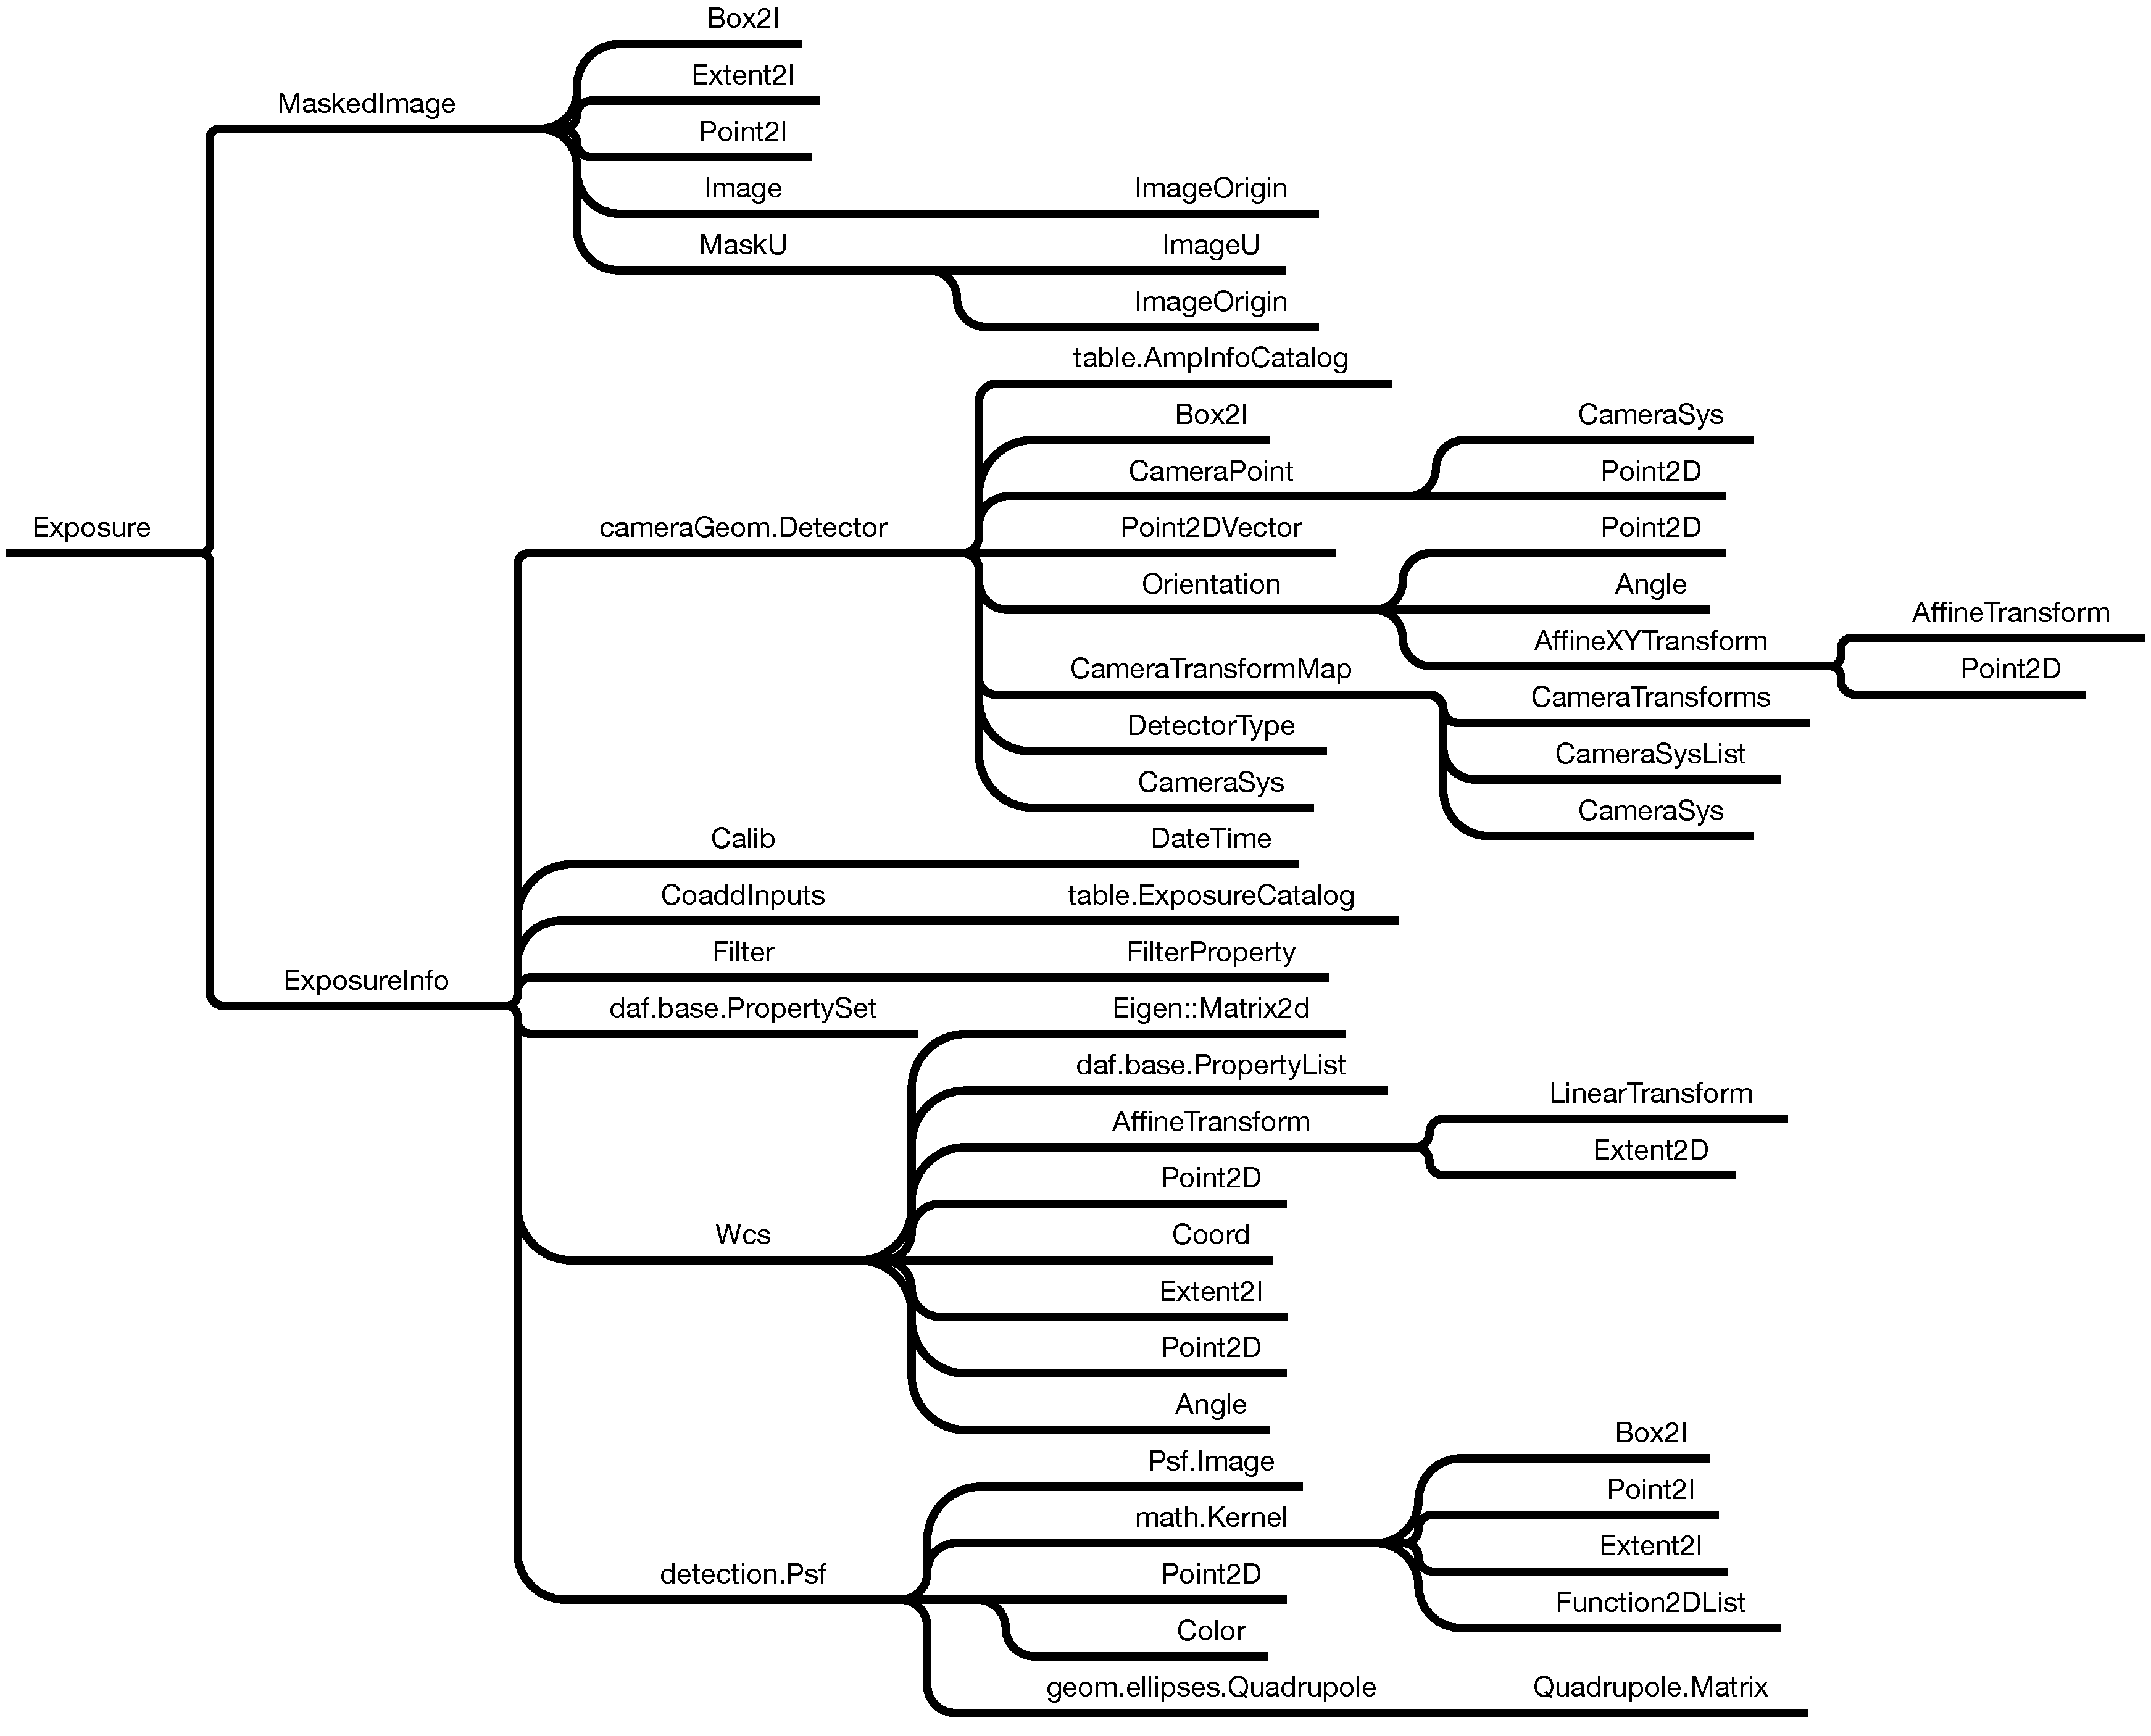
\includegraphics[width=\textwidth]{exposure-dependencies}
\end{center}
\caption[layers]
%>>>> use \label inside caption to get Fig. number with \ref{}
{\label{fig:exposure}
The LSST classes that are used to define a \texttt{lsst.afw.image.Exposure}.}
\end{figure}

\section{Suggested modifications to LSST}
\label{sec:lsstmods}

In addition to working with the Astropy community, there is also the question of how integrated the LSST software system should be with Astropy.
This covers the adoption of distribution standards and use of Astropy classes in our codebase.
These changes will result in a more supportable and sustainable codebase allowing LSST to focus on core deliverables without having to support general infrastructure.
In this section we explore the areas where the LSST software could benefit from adoption of Astropy.

\subsection{Packaging}

\label{sec:packaging}

The LSST data management software uses the EUPS tool\cite{EUPS} to manage versions and dependencies.
It is used to ensure that the versions of all packages used for a particular processing run can be assigned a single number and also to track the packages that were part of a single build.
Development versions can easily be included along with versions from builds done in the past.
This can significantly simplify debugging cycles and aid with provenance tracking but it is a complex environment with a steep learning curve and most users of LSST software outside of the data center and LSST developer community do not need this power.
EUPS can be thought of as a more powerful Python virtual environment where each package can have a specific version enabled to allow mixing and matching of multiple packages, rather than just having entire installations in different virtual environments.

LSST packages are built using the SCons tool\cite{2005Scons1377085}.
SCons is an alternative tool to Make and CMake that is written entirely in Python.
This allows developers to use Python for their library code and build system whilst making use of the powerful source code dependency tracking provided by SCons to prevent wasteful recompilation of files that have not been affected by local edits.

The majority of the Python community have adopted a build system based around the convention of a \texttt{setup.py} file that can be executed to do the build.
This file uses \texttt{distutils} or \texttt{setuptools} to determine what should be built and can handle most cases where external C/C++ code should be compiled into the Python package.
There is a strong expectation that any packages made available to the Astropy community should follow the standard Python build convention of supporting \texttt{python setup.py build} and this is a requirement if we wish to make some LSST packages \emph{Astropy affiliated packages}.
This also allows packages to be distributed on the Python Package Index (PyPI\footnote{\url{https://pypi.python.org}}) providing the ability for a general user to use \texttt{pip install lsst\_apps} to install the LSST software.

As a proof of concept we have demonstrated that an LSST package using the standard LSST directory layout can be built using \texttt{setuptools}.
EUPS is used to determine dependencies and this information can be converted to a standard \texttt{setuptools} dependency request.
To get this working on PyPI it is necessary either to generate the \texttt{setup.py} using a SCons target or else use EUPS directly in the \texttt{setup.py}.
The latter would require that EUPS is also available from PyPI (it currently is not) but might be less prone to errors.

\subsection{Astronomical Coordinates}

The LSST \texttt{afw.coord} package provides coordinate conversions between ICRS, FK5, Galactic, ecliptic and topocentric coordinate systems.
It is written in C++ and has no external dependencies on standard coordinate libraries.
The \texttt{astropy.coordinates} package provides a very usable Python API on top of the standard ERFA astrometry C library\footnote{ERFA is a relicensed version of the standard SOFA library\cite{2011SchpJ...611404H}.}.
It supports all the coordinate systems provided by the LSST package and many more including FK4.

The LSST C++ code does not use any system other than ICRS; therefore we are proposing to remove this package and replace it with a simple spherical coordinates class.
All the Python code will then be modified to use \texttt{astropy.coordinates} and at the Python/C++ boundary coordinates will be converted to/from ICRS.

\subsection{Tables}

LSST and Astropy both have table libraries, but these have different data models and hence different strengths.
LSST's are better for row-based access and provide a limited ORM layer that's valuable for pipeline use when the columns are known in advance and data are appended to the table, while Astropy's excel at column-based access and use in interactive analysis.
Furthermore, Astropy tables now support export to pandas DataFrames\cite{mckinney-proc-scipy-2010}, opening up a richer environment for query-based analysis.
However, the LSST and Astropy table data models are similar enough to allow read-write, memory-sharing Astropy views to LSST tables to be constructed in Python, and a proof-of-concept implementation of this functionality has already been developed.
As this view interface improves, consumers of table-based LSST data products will be able to simply use Astropy tools for analysis, removing much of the need for LSST to develop its own support for many table operations.

\subsection{C++ Bindings}

The LSST Data Management team adopted SWIG as the standard method for providing a Python interface to the C++ code.
Astropy has adopted Cython\cite{2010/content/aip/journal/cise/13/2/10.1109/MCSE.2010.118} when it is required to call C code.
The Astropy core libraries currently do not call C++, and while Cython support for C++ exists, this support is relatively new and somewhat experimental.
The Astropy project has no hard rules concerning how C/C++ code should be included in an affiliated package but has a strong preference for Cython.
LSST is not averse to switching away from SWIG (which results in massive code bloat and extended compile times as currently implemented) and has agreed to investigate Cython\cite{dmtn-013} and pybind11\cite{dmtn-014}\footnote{\url{http://pybind11.readthedocs.org/}}.
One critical requirement is that any move away from SWIG we must be able to do so in an incremental way and so it must be possible for a C++ object produced from SWIG to be passed into a C++ interface created with the new approach.
This has been demonstrated successfully as part of the Cython and pybind11 investigations.

\subsection{Quantities and Units}

With the exception of an angle class, LSST does not use any unit conversion machinery.
Astropy's \texttt{Quantity}, a value with an associated unit, is a very powerful class that can remove an entire category of bugs from scientific software by ensuring that mathematical operations between quantities use compatible units.
The units package in Astropy has been adapted from the units classes in the \texttt{pynbody} analysis module\cite{pynbody}.
For heavily used public APIs it would seem to be clear that arguments should be quantities wherever possible.
The question for LSST is how far down in the stack quantities should be used given the performance hit associated with quantities over plain variables.
Additionally, how much more complicated does the C++/python interface become if SWIG has to be taught how to convert quantities to the correct form before passing the value to the C++.
This is especially critical for large arrays, supplied externally, being passed through where we do not want to do a copy operation before entering C++ and also do not want to normalize units for millions of data points at that time.
Large data arrays and, in particular, table columns returned from C++ layers would benefit from being returned as quantities, as this gives much more flexibility to users of the data and minimizes the risk of misinterpretation of values if units are later changed for a column or the user relies entirely on documentation to interpret values.
The proposal is that LSST software adopts quantities on a case-by-case basis, and its developers will be continuously on the lookout for any performance impact associated with quantities.

\subsection{Time}

LSST uses a C++ time class, \texttt{lsst::daf::base::DateTime} to provide basic time conversion functionality for Modified Julian Dates and UTC.
The Astropy \texttt{astropy.time} package has far more functionality and adopting it in Python LSST code is quite attractive.
The complication is in how to make a Python view of a \texttt{daf\_base} time object look like an \texttt{astropy.time} and vice versa when crossing the Python/C++ boundary.
One way forward may be to implement the C++ class using \texttt{astropy.time} objects.
An experimental implementation does exist demonstrating that this can be made to work, although more experimentation is required.
In particular, Python calling C++ that calls Python can be relatively brittle and can break if there is a Python shared library mismatch.
Also, C++ calling Python in a loop will be much slower than calling C++ and the C++ caller could be surprised by a big performance change if the implementation of the C++ library is changed to use Python.

\section{Proposal}

The concrete proposals from this investigation are therefore:

\begin{itemize}
\item Change EUPS packaging to use a \texttt{setup.py} and upload it to PyPI.
\item Investigate the addition of a \texttt{setup.py} for standard LSST Python packages in addition to our current Scons-based build system.
\item Support views of LSST tables as Astropy tables.
\item Determine whether STC-2, in YAML form, is a suitable basis for WCS interoperability.
\item Remove LSST astronomical coordinate classes and replace with Astropy coordinates in Python and a generic spherical coordinates class in C++.
\item Consider using \texttt{astropy.time}, even in C++.
\item Investigate migration away from SWIG for C++ bindings.
\item Contribute the LSST \texttt{Footprint} code to Astropy.
\item Create an Astropy affiliated package from the \texttt{afw.detection} package.
\item Investigate rationalizing of LSST and Astropy spherical geometry region handling.
\item Modify \texttt{Exposure} to implement an \texttt{NDData}-like interface.
\item Work with the Astropy project to add required functionality such as pixel origins to \texttt{NDData}.
\item LSST will allow Astropy quantity objects to be used in public interfaces on a case by case basis.

\end{itemize}

With these changes implemented LSST will have a solid base from which to assess whether it is feasible to migrate more LSST code to the community as affiliated packages.
It is probable that LSST will start to migrate the existing codebase entirely to Astropy classes where appropriate classes exist.
In particular \texttt{astropy.coordinates} could be adopted fairly rapidly.
Switching time libraries may require significantly more thought.

\section{Conclusion}

The LSST project has a code base that has developed over a number of years and has been developed independently of the wider Python astronomy software community.
We have looked at the Astropy package and worked with the Astropy team to understand areas where synergies exist and where LSST can contribute more fully to the community without delaying our primary deliverables.
The proposals outlined in this document go a long way towards integrating LSST into the wider software community and should bring key benefits to LSST and research astronomers.
Work on these changes has already begun and the intent is to allocate significant effort to this migration in the second half of 2016.

\acknowledgments\

We thank those who attended the LSST/Astropy Summit at the University of Washington in March 2016 that forms the basis for the approaches outlined in this paper.
This material is based upon work supported in part by the National Science Foundation through Cooperative Support Agreement (CSA) Award No.\ AST--1227061 under Governing Cooperative Agreement 1258333 managed by the Association of Universities for Research in Astronomy (AURA), and the Department of Energy under Contract No.\ DE--AC02--76SF00515 with the SLAC National Accelerator Laboratory.
Additional LSST funding comes from private donations, grants to universities, and in-kind support from LSSTC Institutional Members.

% References
\bibliography{lsst-astropy} % bibliography data in report.bib
\bibliographystyle{spiebib} % makes bibtex use spiebib.bst

\end{document}
